\documentclass[12pt,a4paper,uplatex]{jsarticle}
\usepackage[utf8]{inputenc}
%\usepackage{graphicx}
%\usepackage{bm}
%\usepackage{amsmath}

\usepackage[T1]{fontenc}
\usepackage{ascmac, here, txfonts, txfonts}
\usepackage{listings, jlisting}
\usepackage{color}
\usepackage{fancybox}
\usepackage{comment}
\usepackage[dvipdfmx]{graphicx}
\usepackage {colortbl,array,xcolor}
\usepackage{framed}
\usepackage {boites}
\usepackage{eclbkbox}
\usepackage{url}

\lstset{
	%プログラム言語(複数の言語に対応,C,C++も可)
	language = Java,
	%背景色と透過度
	backgroundcolor={\color[gray]{.90}},
	%枠外に行った時の自動改行
	breaklines = true,
	%自動改行後のインデント量(デフォルトでは20[pt])	
	breakindent = 12pt,
	%標準の書体
	basicstyle = \ttfamily\scriptsize,
	%コメントの書体
	commentstyle = {\itshape \color[cmyk]{1,0.4,1,0}},
	%関数名等の色の設定
	classoffset = 0,
	%キーワード(int, ifなど)の書体
	keywordstyle = {\bfseries \color[cmyk]{0,1,0,0}},
	%表示する文字の書体
	stringstyle = {\ttfamily \color[rgb]{0,0,1}},
	%枠 "t"は上に線を記載, "T"は上に二重線を記載
	%他オプション:leftline,topline,bottomline,lines,single,shadowbox
	frame = TBrl,
	%frameまでの間隔(行番号とプログラムの間)
	framesep = 5pt,
	%行番号の位置
	numbers = left,
	%行番号の間隔
	stepnumber = 1,
	%行番号の書体
	numberstyle = \tiny,
	%タブの大きさ
	tabsize = 4,
	%キャプションの場所("tb"ならば上下両方に記載)
	captionpos = none
}

\renewcommand{\lstlistingname}{}

\setcounter{secnumdepth}{6}
\setcounter{secnumdepth}{6}

% Title Page
\title{Remote Sensor Project}
\author{S.Matoike}


\begin{document}
\maketitle

\tableofcontents

%\begin{abstract}
%\end{abstract}

%\chapter{リモート計測システム}

\section{リモートマシン}

\subsection{リモート機器、センサー}

\begin{figure}[H]
	\begin{minipage}[b]{0.45\linewidth}
		\centering
		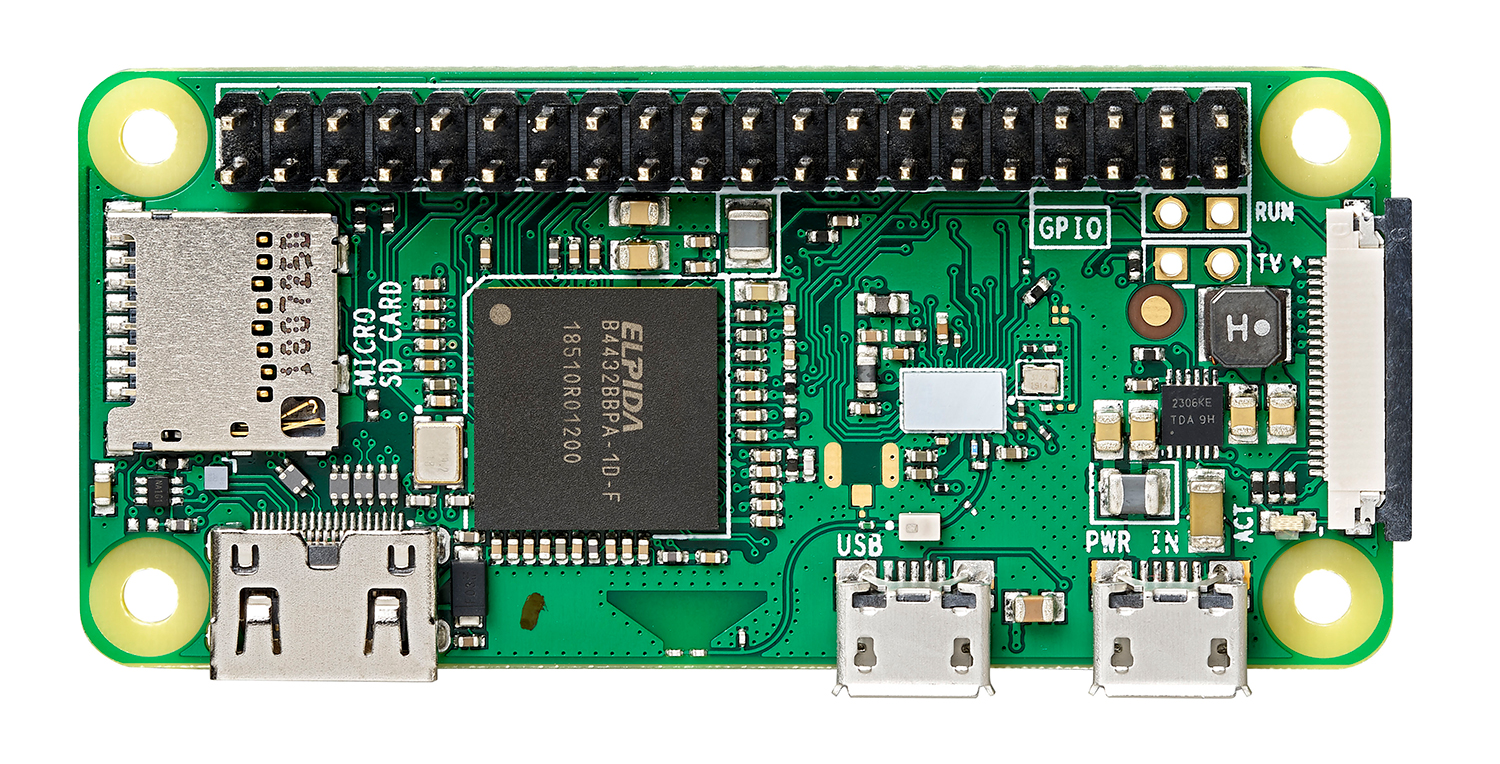
\includegraphics[keepaspectratio, scale=0.13]{figs/jpg/udrpzwh.jpg}
		\caption{Raspberry Pi Zero WH}
	\end{minipage}
	\hspace{1.0cm}
	\begin{minipage}[b]{0.45\linewidth}
		\centering
		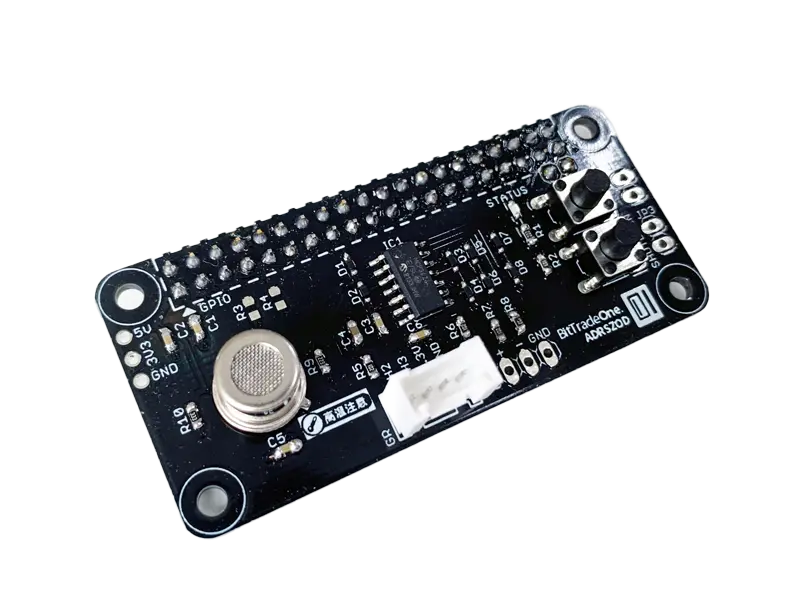
\includegraphics[keepaspectratio, scale=0.25]{figs/png/nioi_sensor.png}
		\caption{ADRSZOD:TP401A}
	\end{minipage}
\end{figure}

\subsection{リモート処理の概要}

\begin{itemize}
	\item Raspberrin Pi Zero WH 上に用意したこのshell(sensor.sh)は、別のRaspberryPiマシンからsshによって起動される
	\item i2Cで接続された臭気センサの出力(電圧値)は、Pythonのプログラム(adrszOD.py)によって読み取ることができる
	\item adrszOD.pyはch1からch4までの値を出力しているので、その出力をawkにパイプして、1つ目のch1の値だけを取り出している
	\item dateコマンドで作成している測定日付は、後ほどPythonのmatplotlibの都合に合わせて、新たにデータの整形処理が必要になることのない様、書式を「年−月−日と時:分:秒の間は、半角カンマ+半角スペース1個」の格好になるように整形している
	\item 日付とセンサの出力する値が1行になる様にするため、pasteコマンドを使っている
	\item paste の2つのオペランド、<(date +....) と、<(python3 adrszOD.py...)の各々のコマンドを、<(any command) の形に囲むことにより、2つのファイルの様に扱うことができる(プロセス置換\footnote{「Efficient Linuxコマンドライン」オライリー・ジャパン 初版第1刷のp.156に、プロセス置換の解説がある})
\end{itemize}

\begin{itembox}[l]{/home/mat/Documents/sensor.sh}
	\begin{verbatim}
#!/usr/bin/bash
dir='/home/mat/Documents'
paste <(date +%Y-%m-%d,\ %H:%M:%S) \
<(python3 "${dir}"/adrszOD.py | awk '{print $1}')
	\end{verbatim}
\end{itembox}

\begin{itembox}[l]{sensor.sh の出力例}
	\begin{verbatim}
mat@raspberrypizero:~/Documents $ ./sensor.sh 
2024-04-17, 02:40:55	ch1:0.79827
mat@raspberrypizero:~/Documents $ 
	\end{verbatim}
\end{itembox}

\begin{itembox}[l]{/home/mat/Documents/adrszOD.py}
	\begin{verbatim}
#!/usr/bin/env python
import smbus
import time

i2c = smbus.SMBus(1)
addr=0x68
Vref=2.048

def swap16(x):
  return (((x << 8) & 0xFF00) | ((x >> 8) & 0x00FF))

def sign16(x):
  return ( -(x & 0b1000000000000000) | (x & 0b0111111111111111) )

def readval(x):
  i2c.write_byte(addr, x) #16bit
  time.sleep(0.2)
  data = i2c.read_word_data(addr,0x00)
  raw = swap16(int(hex(data),16))
  raw_s = sign16(int(hex(raw),16))
  volts = round((Vref * raw_s / 32767),5)
  return volts

if __name__=="__main__":
  volts1 = readval( 0b10011000 )
  volts2 = readval( 0b10111000 )
  volts3 = readval( 0b11011000 )
  volts4 = readval( 0b11111000 )
  out_msg = 'ch1:' + str(volts1) + ' ,ch2:' + str(volts2)+\
    ' ,ch3:' + str(volts3)+ ' ,ch4:' + str(volts4)
  print(out_msg)
	\end{verbatim}
\end{itembox}

\section{ローカルマシン}

\subsection{ローカル機器}

\begin{figure}[H]
	\begin{minipage}[b]{1.0\linewidth}
		\centering
		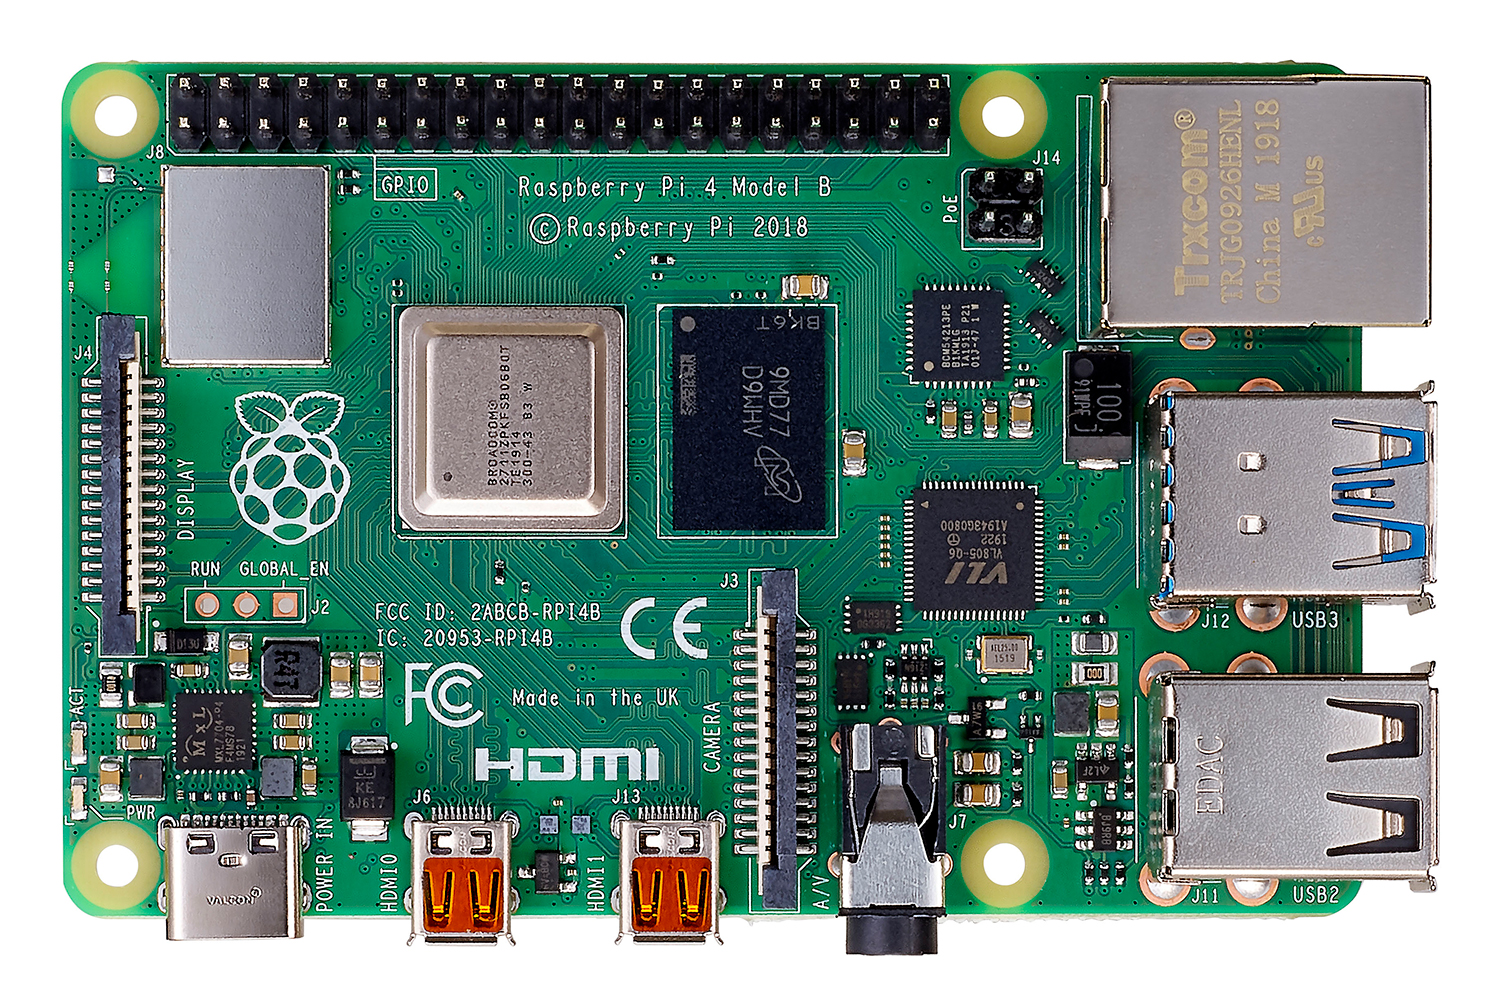
\includegraphics[keepaspectratio, scale=0.12]{figs/jpg/udrp4b_front.jpg}
		\caption{Raspberry Pi}
		%	\end{minipage}
	%	\hspace{1.0cm}
	%	\begin{minipage}[b]{0.45\linewidth}
		%		\centering
		%		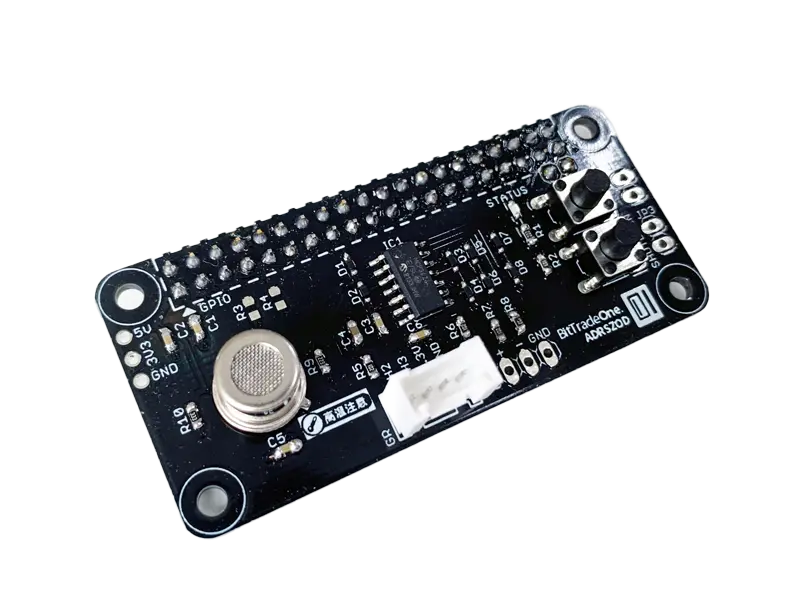
\includegraphics[keepaspectratio, scale=0.25]{figs/png/nioi_sensor.png}
		%		\caption{ADRSZOD:TP401A}
	\end{minipage}
\end{figure}

%\subsection{処理の概要}

\subsection{cronによる時刻指定の処理}

cronの仕組みを使うことにする(3つの時刻指定の処理を登録している)
\begin{enumerate}
	\item[(1)] 5分ごとに、リモートセンサの値を読み取る処理、rsensor.sh を起動する
	\item[(2)] 毎日23時56分になったら、その日1日分の測定データを退避する処理、dayly.sh を起動する
	\item[(3)] 毎週日曜日の朝0時1分になったら、先週1週間の(先週の日曜日の0時0分から昨日の土曜日の23時55分まで5分間隔で測定した)測定データをまとめる処理、weekly.sh を起動する
\end{enumerate}

\begin{itembox}[l]{crontab -e}
	\begin{verbatim}
		MAILTO=""
		*/5 * * * * sh /home/mat/Documents/rsensor.sh
		56 23 * * * sh /home/mat/Documents/dayly.sh
		1 0 * * Sun sh /home/mat/Documents/weekly.sh
	\end{verbatim}
\end{itembox}

ここで、MAILTO="" としているのは、「指定時刻にcronが処理を起動したよ」というメールを送信するためにsmtpを起動しようとして失敗し、指定の処理が起動されないという現象に対する対応である\footnote{postfixやsendmailなど、SMTPの何某かをインストールせよという説もあるが、特にメールの知らせが不要ならこのやり方が最も簡易な解決方法になる}

\begin{screen}
	\begin{verbatim}
		+---------------- minute (0 - 59)
		|  +------------- hour (0 - 23)
		|  |  +---------- day of month (1 - 31)
		|  |  |  +------- month (1 - 12)
		|  |  |  |  +---- day of week (0 - 6) (Sunday=0 or 7)
		|  |  |  |  |
		*  *  *  *  *  command to be executed
	\end{verbatim}
\end{screen}

\newpage

\subsection{リモートセンサの処理をローカルマシンから起動する}

リモート(192.168.3.27)のRaspberry Pi Zero WH に接続されている臭気センサの値を読みとるshell(sensor.sh)を、ローカル(192.168.3.21)のマシンRaspberry Pi からssh を使って起動するための shell(rsensor.sh)であり、cronによって5分ごとに起動される

この時sshから、リモートマシン(Pi Zero)のユーザ(今の環境ではmat)のパスワードを要求されるが、人手によるインタラクティブな入力操作を想定していないので、予めsshpassを導入しておいて、それによってパスワードを自動応答させる様にしている

sshでリモートのshellを実行した結果を受け取り、ローカルのw.txtに追記し蓄積していっている

\begin{itembox}[l]{/home/mat/Documents/rsensor.sh}
	\begin{verbatim}
#!/usr/bin/bash
### sudo apt install -y sshpass ###
dir='/home/mat/Documents'
addr='192.168.3.27'
usr='mat'
pwd='mypassword'
sshpass -p "${pwd}" ssh "${usr}"@"${addr}" "${dir}"/sensor.sh \
>> "${dir}"/w.txt
	\end{verbatim}
\end{itembox}

w.txtの様子は、tail -f w.txt などとしてみると、5分ごとに起動されたshell(rsensor.sh)によって、測定結果が蓄積されていく様子がわかる(このファイルは、1日の終わりの処理で 2024-04-16.txt の様に、日付をつけたファイル名に変えて保存している)

\begin{itembox}[l]{w.txt -> 2024-04-16.txt}
	\begin{verbatim}
		2024-04-16, 00:35:04	ch1:1.0896
		2024-04-16, 00:40:04	ch1:1.09016
		2024-04-16, 00:45:04	ch1:1.09322
		.... ....
		2024-04-16, 23:45:04	ch1:0.9059
		2024-04-16, 23:50:04	ch1:0.99653
		2024-04-16, 23:55:04	ch1:0.98809
	\end{verbatim}
\end{itembox}

\subsection{日毎の処理}

毎日の23時55分に、その日の最後の測定が終わる事を前提として、cronには23時56分になったら次のshell(dayly.sh)を起動する様にしている

現在時刻が23時55分を超えていることを確認した上で、次のことを行っている
\begin{itemize}
	\item 蓄積された1日分の測定データ w.txt を、bkup.txt という名前のファイルにコピーしている
	\item w.txt を、dataフォルダ以下に、「今日の日付.txt」 という名前に変更して保存している
	\item 空のファイル w.txt を次の日の測定データの蓄積場所のために用意している( touch)
	\item Pythonの仮想環境venv11に入って、dayly.py を起動している(第1引数にdataフォルダ以下に保存した測定データファイルの名前=年月日を指定している)
	\item プログラムの実行を終えたら、Pythonの仮想環境venv11から抜けている
\end{itemize}

\begin{itembox}[l]{/home/mat/Documents/dayly.sh}
	\begin{verbatim}
#!/usr/bin/bash
dir='/home/mat/Documents'
dates=`date +%Y-%m-%d`
hour=`date +%H`
minu=`date +%M`
if [ "${hour}" -ge 23 ]; then
  if [ "${minu}" -gt 55 ]; then
    cp "${dir}"/w.txt "${dir}"/bkup.txt
    mv "${dir}"/w.txt "${dir}"/data/"${dates}".txt
    touch "${dir}"/w.txt
    source "${dir}"/venv11/bin/activate
      "${dir}"/venv11/bin/python3 "${dir}"/dayly.py "${dates}"
    deactivate
  fi
fi
	\end{verbatim}
\end{itembox}

%\newpage

\subsection{日毎処理のプログラム}

\begin{itemize}
	\item myplot.py から、graph\_plot() 関数をimport している(この関数の詳細は後述)
	\item 第1引数に指定があったら、そこで指定された日付のデータを元に、グラフを描画できる様にしている
	\item 指定のデータファイルを開いて、最初の20文字までは、予めmatplotlibのdatesに対応した様式の日付文字列にしているので、それをUnixの日付けに変換している
	\item 25文字目以降は、測定した電圧の値だが、改行文字が付いていたりするので、.strip()によってホワイトスペースを除去して、実数に変換している
	\item 日付と電圧のリストを作って、それをgraph\_plot()関数に渡して作図させている
\end{itemize}

\begin{itembox}[l]{/home/mat/Documents/dayly.py}
	\begin{verbatim}
import sys
from datetime import datetime as dt
import matplotlib.dates as mdates
from myplot import graph_plot

dirstr = '/home/mat/Documents'
today = dt.now().strftime('%Y-%m-%d')
if len(sys.argv) > 1:
  today = sys.argv[1]

list0=[]
with open(dirstr + "/data/" + today + ".txt") as f:
  for line in f:
    datestr = line[:20].strip()
    datev = mdates.datestr2num(datestr)
    value = float(line[25:].strip())
    list0.append([datev, value])

graph_plot(list0, dirstr, today, False)
	\end{verbatim}
\end{itembox}

\newpage

このPythonのプログラムを実行した結果として、次の様な1日分のデータの変化をグラフ化したものが得られる(これはfigsフォルダ以下に 「今日の日付.png」 という名称で保存している)

\begin{figure}[htbp]
	\begin{minipage}[b]{1.0\linewidth}
		\centering
		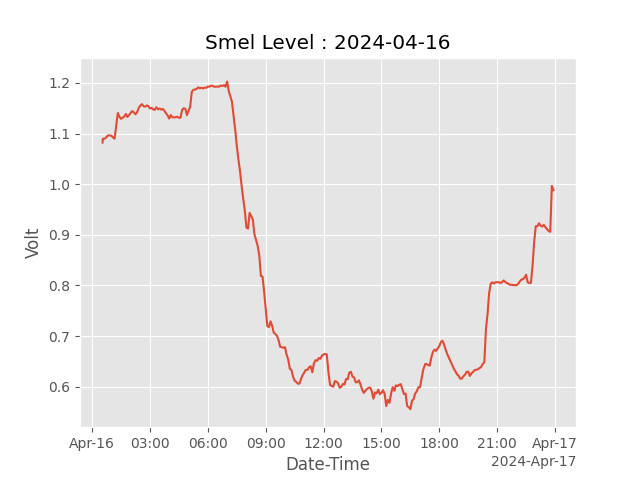
\includegraphics[keepaspectratio, scale=0.8]{figs/png/2024-04-16.png}
		\caption{dayly.pyの出力(4月16日の0時から24時まで)}
	\end{minipage}
	%\hspace{1.0cm}
	%\begin{minipage}[b]{0.45\linewidth}
	%\centering
	%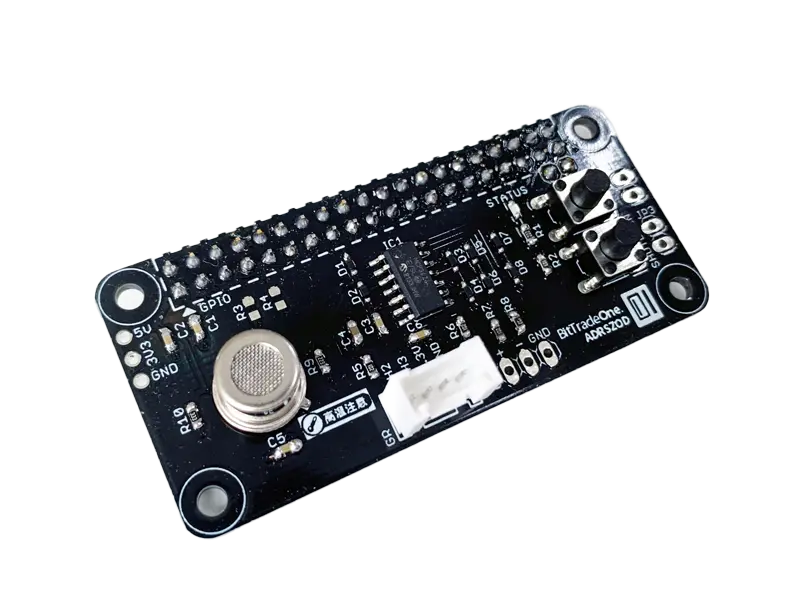
\includegraphics[keepaspectratio, scale=0.25]{figs/png/nioi_sensor.png}
	%\caption{ADRSZOD:TP401A}
	%\end{minipage}
\end{figure}

\subsection{グラフ描画のための関数(myplot.py)}

dayly.py と weekly.py で共通に呼び出しているgraph\_plot()関数を定義している

横軸に日付と時刻(データは5分毎)を置くため、少し工夫が必要になる

ポイントは、matplotlibが理解する日付の様式で書いたものを使うと、matplotlibのdatesに、locatorとformatterを自動生成させて、それ以下の全てを任せきることができる\footnote{\url{https://matplotlib.org/stable/api/dates_api.html}
	の記事が参考になる}

\begin{itembox}[l]{/home/mat/Documents/myplot.py}
	\begin{verbatim}
		import numpy as np, pandas as pd
		from matplotlib import pyplot as plt, style, dates as mdates
		
		def graph_plot(list0, dirstr, datestr, weekly=False):
		  df = pd.DataFrame(list0, columns=["DateVal", "Value"])
		  matplotlib.style.use('ggplot')
		  fig, ax = plt.subplots()
		  x = df.loc[:,"DateVal"].values
		  y = df.loc[:,"Value"].values
		  locator = mdates.AutoDateLocator()
		  formatter = mdates.ConciseDateFormatter(locator)
		  ax.xaxis.set_major_locator(locator)
		  ax.xaxis.set_major_formatter(formatter)
		  ymax = np.array([y.max(), 1.45]).max()
		  ymin = np.array([y.min(), 0.25]).min()
		  ax.set_ylim([ymin, ymax])
		  ax.set_xlabel('Date-Time')
		  ax.set_ylabel('Volt')
		  if weekly:
		    titlestr = "Smel Level : " + datestr + "(Weekly)"
		    figpath = dirstr + "/figs/" + "Weekly_" + datestr
		  else:
		    titlestr = "Smel Level : " + datestr
		    figpath = dirstr + "/figs/" + datestr
		  ax.set_title(titlestr)
		  ax.plot(x,y)
		  fig.savefig(figpath + '.png')
		  plt.show()	
	\end{verbatim}
\end{itembox}

\newpage

\subsection{週毎の処理}

この処理はcronによって、毎週日曜日の朝0時1分に起動される

このshell(weekly.sh)では、0時0分より後の時刻ならば仮想環境venv11に移って、Python のプログラム(weekly.py)を起動し、終わったら仮想環境鵜から抜けている

Pythonのプログラムは、第1引数に日付を受け取ることができる様にしている

\begin{itembox}[l]{/home/mat/Documents/weekly.sh}
	\begin{verbatim}
#!/usr/bin/bash
dir='/home/mat/Documents'
dates=`date +%Y-%m-%d`
hour=`date +%H`
minu=`date +%M`
if [ "${hour}" -ge 0 ]; then
  if [ "${minu}" -gt 0 ]; then
    source "${dir}"/venv11/bin/activate
      "${dir}"/venv11/bin/python3 "${dir}"/weekly.py "${dates}"
    deactivate
  fi
fi
	\end{verbatim}
\end{itembox}

\subsection{週毎処理のプログラム}

\begin{itemize}
	\item myplot.pyからgraph\_plot()関数をimportしている
	\item 第1引数で処理対象にする最終日付を受け取ることができる様にしている
	\item 指定された処理対象の最終日付から、7日前の日付を求めて、7日間の日付のリストdatelistを作っている
	\item 7日間の日付リストdatelistから1日ずつ取り出しては、そのファイル名のデータをdataフォルダから読み出し、日付の変換と電圧の実数への変換を行い、それらのデータのリストをlist0に追記していっている
	\item もし、指定した日付のデータファイルがなかった場合は、例外処理で受けて黙って次の日付のファイルのデータ取得に移る様にしている
	\item graph\_plot()関数にlist0を渡してグラフの作図をさせている
\end{itemize}

\begin{itembox}[l]{/home/mat/Documents/weekly.py}
	\begin{verbatim}
from datetime import datetime as dt, timedelta
import sys, matplotlib.dates as mdates
from myplot import graph_plot

dirstr = '/home/mat/Documents'
s_format = '%Y-%m-%d'
today = dt.now()
if len(sys.argv) > 1:
  today = dt.strptime(sys.argv[1], s_format)
startstr = (today - timedelta(days=7)).strftime(s_format)

datelist = []
for i in range(7):
  day = today - timedelta(days=(7-i))
  datelist.append(day.strftime(s_format))

list0=[]
for fname in datelist:
  try:
    with open(dirstr + "/data/" + fname + ".txt") as f:
      for line in f:
        datestr = line[:20].strip()
        datev = mdates.datestr2num(datestr)
        value = float(line[25:].strip())
        list0.append([datev, value])
  except FileNotFoundError:
    continue

graph_plot(list0, dirstr, startstr, True)
	\end{verbatim}
\end{itembox}

\newpage

以下は、週毎処理が出力する画像である。4月21日(日曜日)の0時1分にcronによって起動され実行されたものだが、フォルダdataの中には、測定を始めた4月16日(火曜日)から、4月20日(土曜日)までの5日分のファイルがあるだけである。本来なら1週間前の日曜日(4月14日)のデータから週毎処理の対象となるところだが、プログラムの中ではFileNotFoundErrorの例外を捕捉して、とにかくcontinueによって処理を継続させているため、何事もなかったかの様に、データファイルの所在する火曜日以降がグラフに作図されている

また、日毎処理のプログラムdayly.pyと全く同じグラフ作図の関数(myplot.pyの中のgraph\_plot()関数)を使っているのだが、横軸の設定がmatplotlibのdates(mdatesとしてプログラム中では使っている)によって、自動的に調整されているのが分かる(便利)

\begin{figure}[htbp]
	\begin{minipage}[b]{1.0\linewidth}
		\centering
		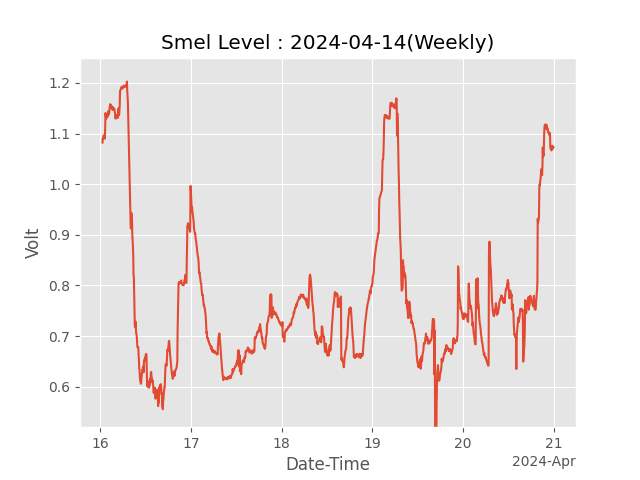
\includegraphics[keepaspectratio, scale=0.8]{figs/png/Weekly_2024-04-14.png}
		\caption{weekly.pyの出力}
	\end{minipage}
	%\hspace{1.0cm}
	%\begin{minipage}[b]{0.45\linewidth}
	%\centering
	%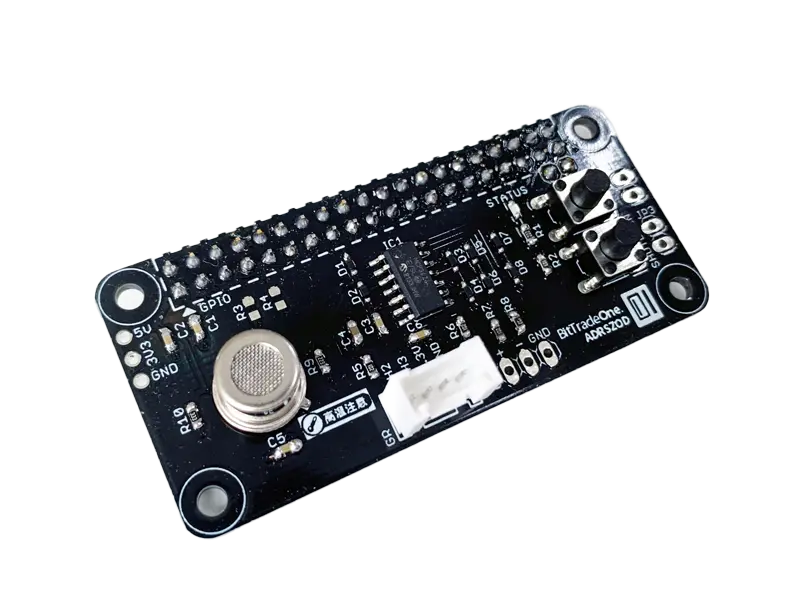
\includegraphics[keepaspectratio, scale=0.25]{figs/png/nioi_sensor.png}
	%\caption{ADRSZOD:TP401A}
	%\end{minipage}
\end{figure}

%\newpage

\subsection{測定データのグラフを実時間で作図する}

\begin{itemize}
	\item RTPlotクラスに必要な関数類をまとめた
	\item ポイントとなるのは、 plt.show() を使わず、plt.pause(1.0)を使うこと、tail -f をプログラム上で実現することの2点である
	\item self.xとself.yのリストに順にデータを追記していき、新たなデータがw.txtに追加されたタイミングでplot.pause(1.0)としている(引数の値を0.1や0.01にするとRaspberry Piでは全て描画しきれないので注意)
	\item tail\_f()関数は、コマンド tail -f w.txt をPythonのプログラムで実現したもの(指定したファイルの最終行が追記されるまでcontinueで待っている)である
\end{itemize}

\begin{breakbox}%[l]{/home/mat/Documents/rtplot.py}
	\begin{verbatim}
import sys, time, numpy as np
from matplotlib import style, pyplot as plt, dates as mdates
from datetime import datetime as dt, timedelta

class RTPlot:
    def dateproc(self):
        #s_format = '%Y-%m-%d, %H:%M:%S'
        s_format0 = '%Y-%m-%d, 00:00:00'
        today = dt.now()
        tomor = today + timedelta(days=1)
        self.todaystr = today.strftime(s_format0)
        self.tomorstr = tomor.strftime(s_format0)

    def readdata(self, fname):
        try:
            with open(fname, 'r') as f:
                for line in f:
                    self.chop(line)
        except FileNotFoundError:
            print(f'File{fname} not found')

    def __init__(self, fname):
        self.fname = fname
        self.x = []
        self.y = []
        self.ims = []
        self.dateproc()
        self.readdata(fname)
        matplotlib.style.use('ggplot')
        self.fig, self.ax = plt.subplots()
        locator = mdates.AutoDateLocator()
        formatter = mdates.ConciseDateFormatter(locator)
        self.ax.xaxis.set_major_locator(locator)
        self.ax.xaxis.set_major_formatter(formatter)
        xmin = mdates.datestr2num(self.todaystr)
        xmax = mdates.datestr2num(self.tomorstr) 
        self.ax.set_xlim([xmin, xmax])
        self.yrange()
        self.ax.set_xlabel('Date-Time')
        self.ax.set_ylabel('Volt')
        self.update()

    def chop(self, line):
        datestr = line[:20].strip()
        datev = mdates.datestr2num(datestr)
        value = float(line[25:].strip())
        self.x.append(datev)
        self.y.append(value)

    def statvalue(self):
        self.ymax = np.array(self.y).max()
        self.ymin = np.array(self.y).min()
        self.mean = np.array(self.y).mean()
        str1 = f"Max={self.ymax:.2f}, Min={self.ymin:.2f}, "
        str2 = f"Mean={self.mean:.2f}"
        self.ax.set_title("Smel Level : " + str1 + str2)

    def tail_f(self):
        try:
            with open(self.fname, 'r') as f:
                f.seek(0, 2)
                enter = dt.now()
                while True:
                    line = f.readline()
                    if not line:
                        time.sleep(1)
                        if dt.now() - enter < timedelta(minutes=6):
                            continue
                        return
                    return line.strip()
        except FileNotFoundError:
            print(f'File{self.fname} not found')
        return

    def yrange(self):
        self.statvalue()
        step = (self.ymax - self.ymin)/10.0
        v = 0
        while self.ymax > v:
            v += step
        ymax = v + step/2.0
        while self.ymin < v:
            v -= step
        ymin = v - step/2.0
        self.ax.set_ylim([ymin, ymax])


    def update(self):
        self.yrange()
        if len(self.ims) > 0:
            im = self.ims.pop()
            im.remove()
        im, = self.ax.plot(self.x, self.y, color='red')
        self.ims.append(im)

if __name__=="__main__":
    dirstr = '/home/mat/Documents'
    fname = dirstr + '/w.txt'
    if len(sys.argv) > 1:
        fname = dirstr + '/' + sys.argv[1]
    rtp = RTPlot(fname)
    tomorrow = dt.strptime(rtp.tomorstr, '%Y-%m-%d, 00:00:00')
    while dt.now() < tomorrow:
        plt.pause(1)
        line = rtp.tail_f()
        if line is not None:
            print("[info.log]", line)
            rtp.chop(line)
            rtp.update()
    rtp.fig.savefig(dirstr+'/figs/R_'+rtp.todaystr[:10]+'.png')
	\end{verbatim}
\end{breakbox}

tail\_f()関数の中では、6分を超えてcontinueを繰り返している場合にNoneを返す事にしている(6分待てば、その間には必ず5分間隔のイベントは入ってくると思う)ので、mainの中の繰り返し処理whileの中でその事を(PEP8が可読性の観点から推奨している書き方) is not None によって判定している

実時間処理の画面は次の様になる.

このプログラム rtplot.py が終了時に保存する画像は、実は日毎処理のプログラム dayly.py が出力するものとほぼ同じ傾向を示しているはずだ。ただ rtplot.py の方は、新たな点をプロットするたびにy軸の最大値と最小値を更新しているため、日毎の処理では作図の範囲外に出るデータも示せているし、また具体的な最大値、最小値、平均値の値もその都度更新して表示している

\begin{figure}[htbp]
	\begin{minipage}[b]{1.0\linewidth}
		\centering
		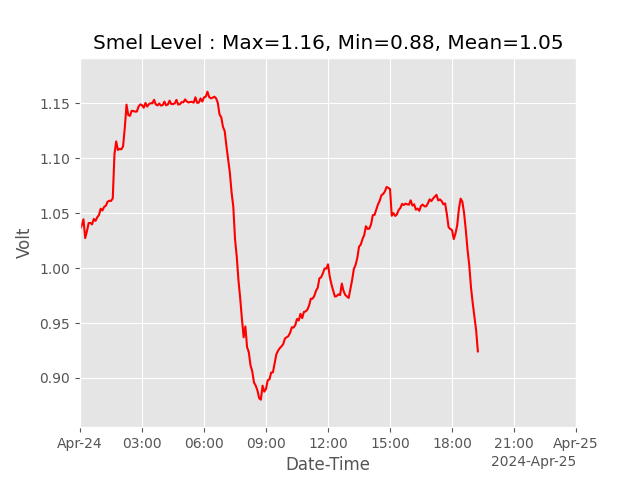
\includegraphics[keepaspectratio, scale=0.8]{figs/png/Figure_5.png}
		\caption{実時間出力の例(途中経過:4月25日の19時過ぎ)}
	\end{minipage}
	%\hspace{1.0cm}
	%\begin{minipage}[b]{0.45\linewidth}
	%\centering
	%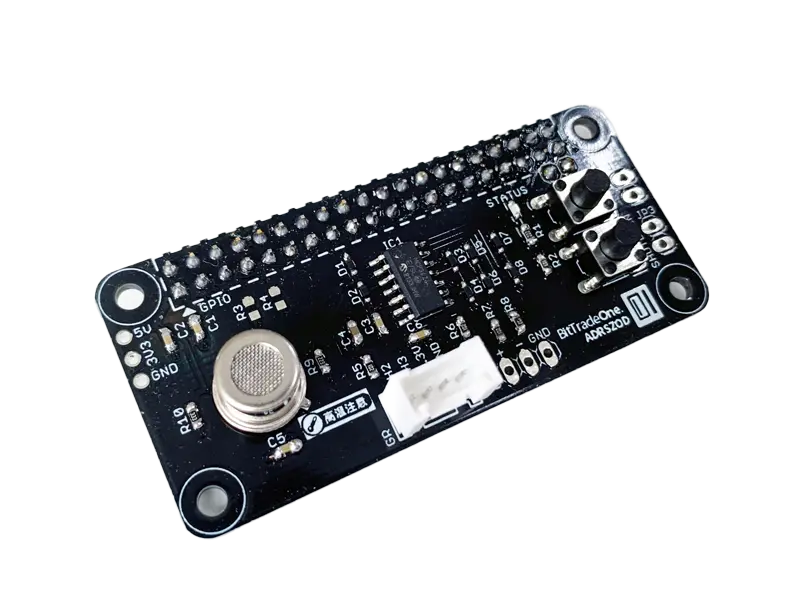
\includegraphics[keepaspectratio, scale=0.25]{figs/png/nioi_sensor.png}
	%\caption{ADRSZOD:TP401A}
	%\end{minipage}
\end{figure}

\newpage

\section{新たなシステムへの移行手順}

\subsection{ローカルマシンの移行}

ここまで作成してきたものを、新たなマシン(Raspberry Pi)へ移行する際、必要になる手続きについてまとめておく
(新しいマシンのOSが導入され、ネットワークの設定を終えた後の手続きになる)

\begin{figure}[htbp]
	\begin{minipage}[b]{1.0\linewidth}
		\centering
		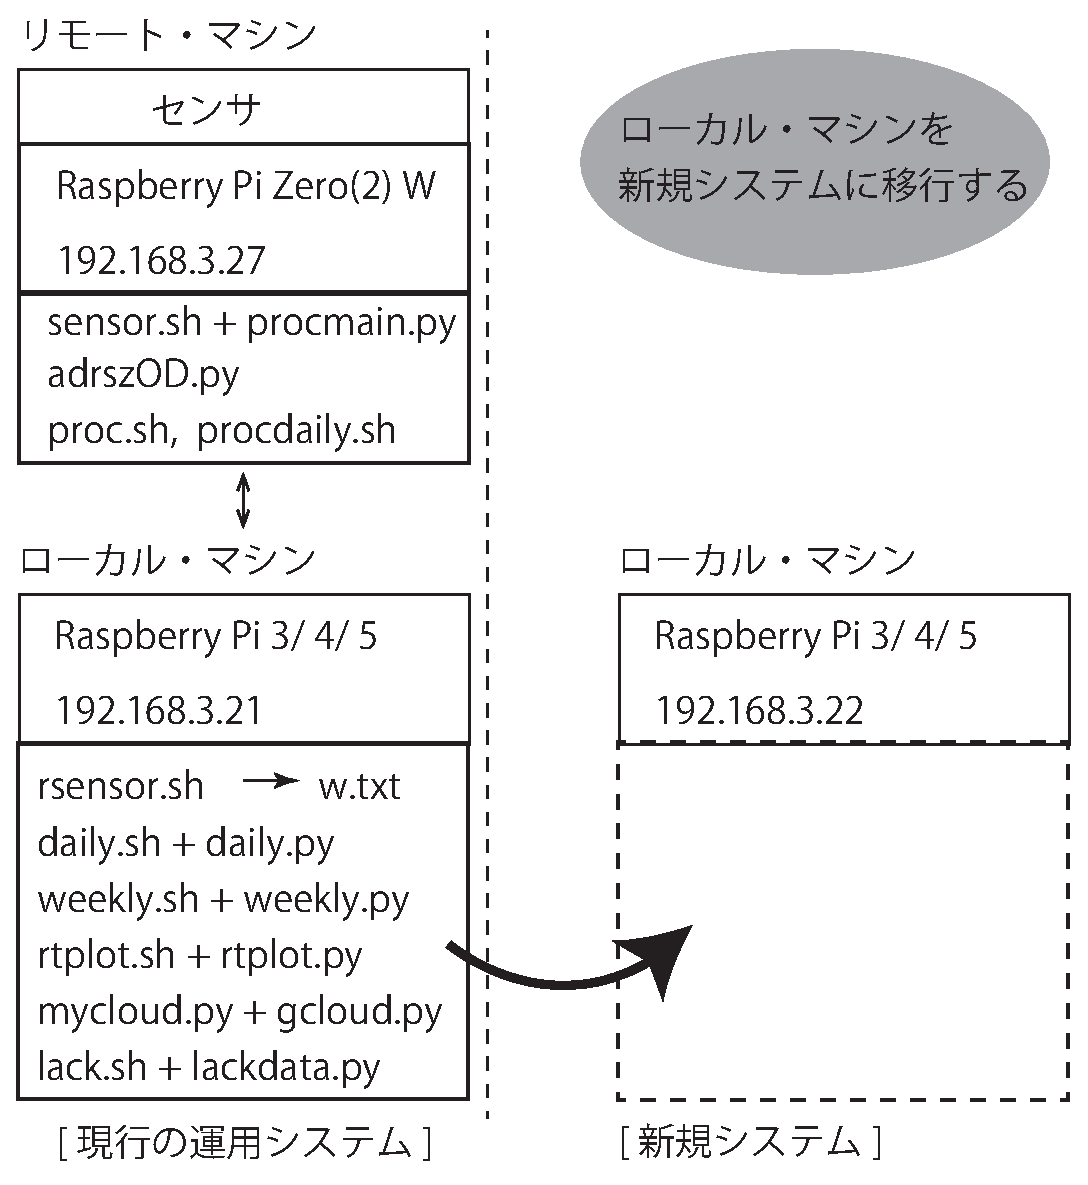
\includegraphics[keepaspectratio, scale=0.4]{figs/eps/ikou.eps}
		\caption{ローカルマシンの移行}
	\end{minipage}
	%\hspace{1.0cm}
	%\begin{minipage}[b]{0.45\linewidth}
	%\centering
	%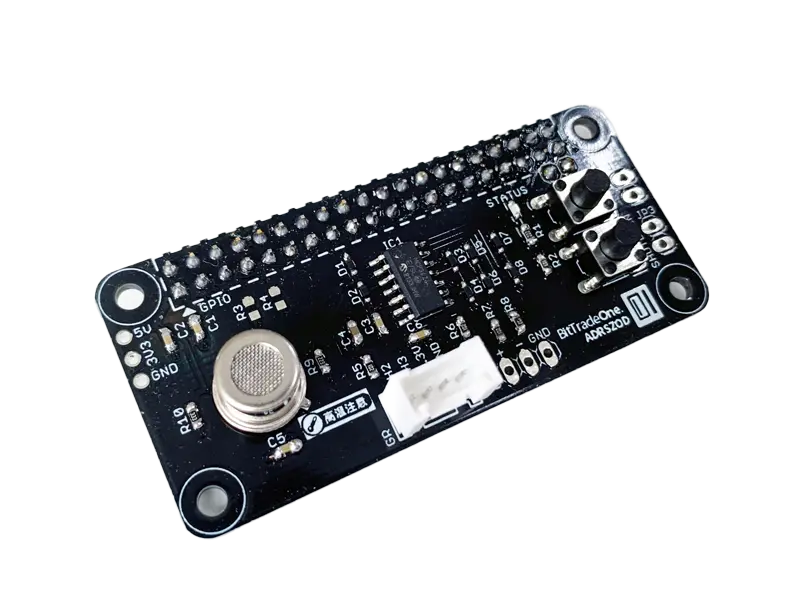
\includegraphics[keepaspectratio, scale=0.25]{figs/png/nioi_sensor.png}
	%\caption{ADRSZOD:TP401A}
	%\end{minipage}
\end{figure}

以下の手続きはその都度全て、/home/mat/Documents の直下で実施するものとする

\begin{enumerate}
	\item sshを有効にする(Raspberry Piのconfigulationで)
	\item システムを最新の状態にする
	\begin{verbatim}
		sudo apt update
		sudo apt dist-upgrade
	\end{verbatim}
	\item sshpass を導入する
	\begin{verbatim}
		sudo apt install -y sshpass 
	\end{verbatim}
	\item Pythonの仮想環境を /home/mat/Documents/venv11 につくる\footnote{寺田学 他3名、翔泳社「Pythonによるあたらしいデータ分析の教科書」第2版、p.50}
	\begin{verbatim}
		python3 -m venv venv11
		source venv11/bin/activate
		python3 -m pip install -U pip
		pip install numpy==1.22.4
		pip install scipy
		pip install pandas==1.4.2
		pip install matplotlib
		pip install scikit-learn
		pip list -o
		deactivate
	\end{verbatim}
	\item dataフォルダとfigsフォルダを移行する
	\begin{verbatim}
		scp -r mat@192.168.3.21:/home/mat/Documents/data ./
		scp -r mat@102.168.3.21:/home/mat/Documents/figs ./
	\end{verbatim}
	\item shellとPythonのプログラムを移行する
	\begin{verbatim}
		scp mat@192.168.3.21:/home/mat/Documents/*.sh ./
		scp mat@192.168.3.21:/home/mat/Documents/*.py ./
	\end{verbatim}
	ここで、各shellには実行可能属性がついている事を確認する ls -l *.sh\\
	もし付いていなかったら付ける chmod +x *.sh\\
	また、リモートマシンのIPアドレス、ユーザ名とそのパスワードが変わる場合は、ここで rsensor.sh の当該箇所(露に記述している)を編集する\\
	Pythonのプログラムに実行可能属性は不要である
	\item cronに時刻指定手続きを登録する(crontab -e)
	\begin{verbatim}
		MAILTO=""
		*/5 * * * * sh /home/mat/Documents/rsensor.sh
		56 23 * * * sh /home/mat/Documents/dayly.sh
		1 0 * * Sun sh /home/mat/Documents/weekly.sh
	\end{verbatim}
	\item sshでリモートマシンに接続を試みて、key fingerprint を登録させる
	\begin{verbatim}
		ssh mat@192.168.3.27
		 The authenticity of host '192.168.3.27' can't be established.
		 ED25519 key fingerprint is SHA256:......
		 This key is not known by any other names.
		 Are you sure you want to continue connecting (yes/no/[fingerprint])? yes
		ssh mat@192.168.3.27 /home/mat/Documents/sensor.sh
	\end{verbatim}
	\item txtファイルを移行する
	\begin{verbatim}
		scp mat@192.168.3.21:/home/mat/Documents/*.txt ./
	\end{verbatim}
	\item rsensor.sh が5分ごとに起動され、w.txt を更新している事を確認する
	\begin{verbatim}
		tail -f w.txt
	\end{verbatim}
	\item 実時間モニタ用のプログラムを起動する
	\begin{verbatim}
		source venv11/bin/activate
		python3 ./rtplot.py
	\end{verbatim}
\end{enumerate}

\subsection{リモートマシンの移行}

新しいリモートマシンへの移行は次の通り\\リモートマシンへのOSの導入とネットワークの設定を終えていること

\begin{enumerate}
	\item configurationで、sshとi2cを有効にする
	\item 最新の状態に更新する
	\begin{verbatim}
		sudo apt update
		sudo apt dist-upgrade
	\end{verbatim}
	\item adrszOD.py を導入する
	\item sensor.sh を導入して、実行可能属性をつける(chmod +x sensor.sh)
	\item /home/mat/Documents/sensor.sh を実行して、現在日時とセンサの電圧、それぞれ適切な値が1行で出力される事を確認する
\end{enumerate}

%\newpage

\section{参考文献}

\begin{itemize}
	\item 臭気センサ拡張基板とそのサンプルプログラム\\
	\url{https://github.com/bit-trade-one/RasPi-Zero-One-Series}
	\item matplotlib が認識する日付の書式\\
	\url{https://matplotlib.org/stable/api/dates_api.html}
	\item プロセス置換\\
	Daniel J.Barrett著、オライリー・ジャパン「Efficient Linuxコマンドライン」初版第1刷、p.157 のコラム記事
	\item Pythonの仮想環境の構築\\
	寺田学 他著、翔泳社「Pythonによるあたらしいデータ分析の教科書」第2版、p.50
\end{itemize}

\end{document}          
